\section{データ転送途上における攻撃}
クラウドサービスでは,他の一般的なインターネット上のサービスと比べ大量のデータを転送するため,それだけユーザとクラウド間の通信時に攻撃を受ける可能性が高い.
したがって,盗聴やなりすましなどの攻撃の持つリスクを十分に考慮しなくてはならない.
そのようなデータ転送中の攻撃への対策として,ユーザがセキュリティ性の高い通信プロトコルや認証方式を用いる方法と,クラウド事業者がセキュアなネットワークを構築するといった方法が考えられる.

\subsection{通信路上の攻撃}
クラウドサービスにおける認証,認可,課金管理(AAA)が不適切であったり,通信路やデータ自体の暗号化が不十分だと,中間者攻撃,なりすまし,サイドチャネル攻撃,リプレイ攻撃などによる通信盗聴といった問題が生じてしまう.

\begin{description}
	\item[中間者攻撃]\mbox{}\\ 
		通信を行う二者の間に割り込んで,両者が交換する公開情報を自分のものとすりかえることにより,
		気づかれることなく盗聴したり,通信内容に介入したりする手法	
	
	\item[リプレイ攻撃]\mbox{}\\
		有効なデータ転送が故意または不正に繰り返し・遅延されることによる攻撃の形式で,
		発信者や攻撃者がデータを傍受し再送信することによって実行される

	\item[サイドチャネル攻撃]\mbox{}\\
		暗号装置の動作状況を様々な物理的手段で観察することにより,
		装置内部のセンシティブな情報を取得しようとする攻撃
		(サイドチャネル攻撃に関しては,次の2.4章で詳しく述べる)
\end{description}

\subsection{ユーザ側の対策}
ここでは,ユーザが攻撃への対策として用いることのできる認証方式やプロトコルについて説明する.
各対策の先に述べた攻撃への対応を図に示す.ここで,サイドチャネル攻撃に関しては対策を行う層が異なるため,ユーザ側の対策としてはどれも当てはまらない.\\

\begin{figure}[h]
 \hspace*{\fill}
 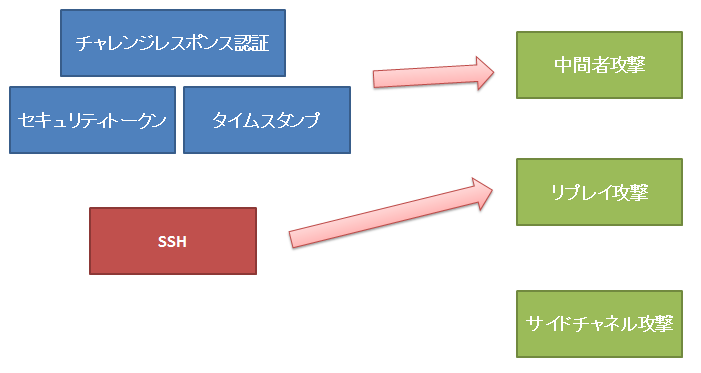
\includegraphics[scale=0.38]{sec}
 \hspace*{\fill}
 \caption{各対策の対象}
\end{figure}

\subsubsection{セキュリティトークン}
セキュリティトークンとは,コンピュータサービスの利用権限のある利用者に,認証の助けとなるよう与えられる物理デバイスのことである.
カードサイズのトークンには,暗証番号を入力するための小さいキーパッドや,ワンタイムパスワードを表示する小さな表示部を備えるものもある.
また,USB端子に挿入して使用するものもあり,その場合は市販のUSBメモリーのような小型のものが多い.
これらのセキュリティトークンは,デジタル署名や,ワンタイムパスワードの信頼性を確保するために用いられることが多い.
トークンのタイプとしては,Bluetooth型,PC・スマートカード型や,USB型のものが挙げられる.
また,携帯電話そのものがセキュリティトークンとして扱われる場合も多い.
セキュリティトークンが携帯電話にインストールされているか,SMSメッセージ交換を使うか,あるいは対話型の電話通信を起こすか,またはhttp・httpsのような標準的なインターネット・プロトコルを使うことで携帯電話認証トークンになり得る.

\subsubsection{SSH(Secure SHell)}
中間者攻撃や盗聴を防ぐためにユーザ側から行える対策としてsshの利用が考えられる.
sshとは,ネットワークを介して別のコンピュータにログインしたり,遠隔地のマシンでコマンドを実行したり,ほかのマシンへファイルを移動したりするためにプログラムに暗号化機能とデータの圧縮転送機能を実装したものである.
通常,UNIX端末のshellをリモートから操作する場合は,パケットの暗号化機能を実装していないため,平文のIPパケットをキャプチャされた場合にオペレーション内容やパスワードを第三者に知られてしまう可能性がある.
そこで通信路全体を暗号化することにより,リモートからのshellでの作業をセキュアにするのがsshということになる.

\subsubsection{チャレンジ・レスポンス認証方式(ワンタイム認証)}
チャレンジ・レスポンス認証とは,認証サーバが「チャレンジ」という毎回変化するランダムなデータをクライアントに送信する.
これを受け取ったクライアントは,チャレンジとユーザのパスワードを基に演算して「レスポンス」というデータを算出し,このレスポンスをサーバに送る.
サーバでは,自身に登録されているパスワードとチャレンジを使って,クライアントと同じ演算でレスポンスを算出し,クライアントから送られてきたレスポンスと照合する.
そして,両者が一致すれば,クライアントのパスワードが正しいと判断し,クライアントを認証するといった方式である.

\subsubsection{タイムスタンプ}
データの送信時間と受信時間にズレがある場合にサーバは受信を拒否する.
また,デジタル署名において,ローカル・マシンのタイムスタンプは信頼性の低いものとして利用されない.
そのため,RFC3161 Time stamp protocolが考案されている.
これは公開鍵基盤PKIを利用するタイムスタンプ認証プロトコルであり,Time Stamping Authority(TSA)と呼ばれる認証局がクライアントから送信されるデータのハッシュを元に"Time-stamp token"を作成,これをクライアントへ応答として返す一連の手続きである.


\subsection{クラウド事業者の対策}
クラウド事業者の運用するネットワークにおける主なセキュリティ対策としては,ゲートウェイを用いた暗号化とトークナイゼーションが挙げられる.

\subsubsection{社内ゲートウェイを用いた暗号化}
クラウド事業者の個人情報を守るための施策として,社内のゲートウェイ経由でクラウドにアクセスし,ゲートウェイ上で個人情報の暗号化と復号を行うことで,データ消失・漏洩のリスクを減らしている.
ここで,暗号化のキーはゲートウェイ側が持っているので,クラウド側では暗号化されたデータを復元できない.
そして,クラウド側ではアクセスログの取得が困難であるが,ゲートウェイを経由するためにそこで取得することができる.

\subsubsection{トークナイゼーション}
トークナイゼーションでは,元データをランダムに発生させたトークンにマッピングし,そのマッピングデータをローカルのデータベースに格納する.
それにより,仮にクラウド上のデータがリスクにさらされたとしても,意味のないデータしか外部に流出しないことになる.
ただし,ローカルにデータベースを持つ必要があるなど運用が難しい点がある.

\subsection{まとめ}
クラウド事業者がセキュリティ対策のために暗号化を用いたシステムなどでデータを扱う一方で,ユーザ側からはクラウドの先,つまりサービス提供者側の技術や運用・管理の実態については見えない.
そのため,ユーザ側でできることとして,最低限通信プロトコルや認証方式に十分注意を払った上でクラウドサービスを利用することが望ましい.しかし,インターネットや情報系の技術に関して詳しくないユーザが完全にそれらを理解することは難しいと考えられる.そのようなユーザを攻撃者からどう守るかが今後の課題となるだろう.
